\section{Hartley}\label{hartley}


\begin{figure}
\centering
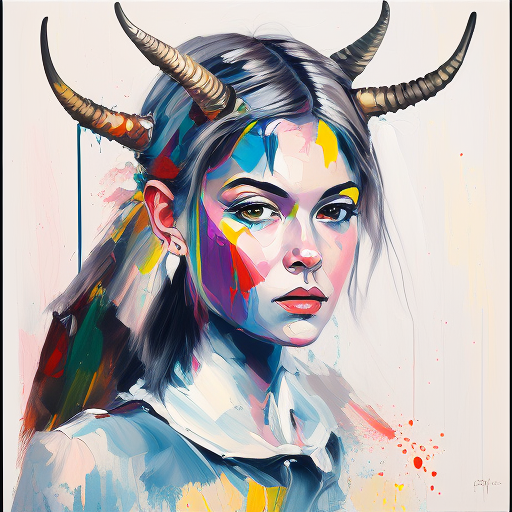
\includegraphics{Hartley_autoritratto.png}
\caption{Hartley\_autoritratto.png}
\end{figure}

Informazioni Generali

Età: 25

Anno di nascita: 1998

Paese di nascita: Kos

Razza: Tiefling

Relazioni:

Alleati:

Nemesi:

Possedimenti importanti:


\subsection{1. Descrizione Generale}\label{descrizione-generale}


\begin{figure}
\centering
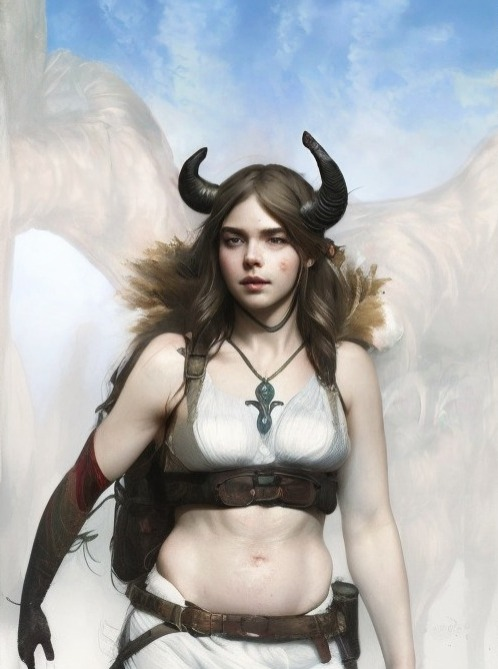
\includegraphics{Hartley.jpeg}
\caption{Hartley.jpeg}
\end{figure}

Lettera di risposta di Marpalo (Quartiermastro dei Protettori di Kos)
alla richiesta di Sitahu di inviare ad Azura un protettore adatto ad una
missione di spionaggio.

``Come mi hai chiesto, ecco tutto quello che so su Hartley Nessuno
conosce la sua vera storia, perché racconta una cosa diversa ogni volta
che qualcuno gliela chiede. A volte è scappata dall'estremo Nord a causa
delle persecuzioni contro i tiefling, altre volte è un'ex prostituta che
ha dovuto uccidere il suo pappone per conquistare la propria libertà,
altre ancora una principessa scappata dal massacro della sua famiglia
durante le rivolte popolari di chissà quale regno lontano. Non
conosciamo neanche il suo cognome, in tasca ha sempre più di un
documento pronto a testimoniare in favore delle sue molteplici
personalità. Probabilmente neanche lei si ricorda più come si chiama.
Bugiarda patologica, ma convincente, mente anche quando non c'è alcun
motivo valido per farlo. Il problema più grande è il suo modo di fare:
sempre cordiale, di buon umore, pronta ad ascoltare e a compatire.
Diresti di lei che è la tua amica più fidata, almeno fino a quando non
riesce ad ottenere da te quello di cui aveva bisogno. Di lei sappiamo
solo che si guadagnava da vivere per strada, distraendo i passanti con
giochi di prestigio e derubandoli mentre lo faceva. Alla fine dello
